\documentclass[preview]{standalone}
\usepackage{tikz}
\begin{document}
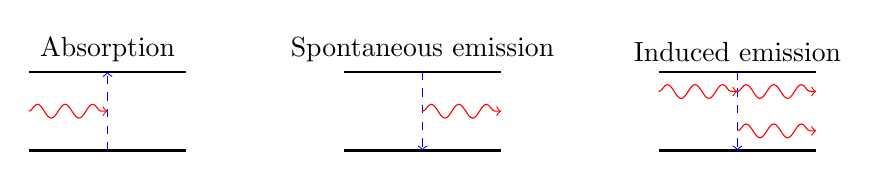
\begin{tikzpicture}


\usetikzlibrary{decorations.pathmorphing}

\tikzset{%
  photon/.style   = {red,decorate,decoration={snake},->},
  electron/.style = {blue,dashed,->},
  border/.style   = {thick},
}

\coordinate(abs)  at (2,0);  % Absorption
\coordinate(spon) at (6,0);  % Spontaneous Emission
\coordinate(ind)  at (10,0); % Induced Emission

% Absorption
\draw[border]   (abs) ++ (0,1) to node[above]{Absorption} ++ (2,0);
\draw[border]   (abs) to ++ (2,0);
\draw[electron] (abs) ++ (1,0) to ++ (0,1);
\draw[photon]   (abs) ++ (0,0.5) to ++ (1,0);

% Spontaneous Emission
\draw[border]   (spon) ++ (0,1) to node[above]{Spontaneous emission} ++ (2,0);
\draw[border]   (spon) to ++ (2,0);
\draw[electron] (spon) ++ (1,1) to ++ (0,-1);
\draw[photon]   (spon) ++ (1,0.5) to ++ (1,0);

% Induced Emission
\draw[border]   (ind) ++ (0,1) to node[above]{Induced emission} ++ (2,0);
\draw[border]   (ind) to ++ (2,0);
\draw[electron] (ind) ++ (1,1) to ++ (0,-1);
\draw[photon]   (ind) ++ (0,0.75) to ++ (1,0);
\draw[photon]   (ind) ++ (1,0.75) to ++ (1,0);
\draw[photon]   (ind) ++ (1,0.25) to ++ (1,0);


\end{tikzpicture}
\end{document}
